\section{Теория}
\subsection{Временные ряды}
Обычно временной ряд - повторяющееся во времени измерение какого-либо параметра с указанием времени, когда измерение было произведено~\cite{time_series_databases}. Временные ряды часто состоят из измерений, производимых через определенный постоянный интервал, но постоянность этого интервала не является обязательной. Например, измерения температуры за последнюю неделю с указанием времени каждого измерения является временным рядом показаний температуры. Временные ряды широко используются в аналитических целях, включая машинное обучение и предиктивную аналитику. Конкретное измерение временного ряда может быть как непосредственно показанием датчика, так и каким-то вычисленным значением, и пока у этого значения есть отметка времени в каком-либо формате, массив таких данных может считаться временным рядом.

\subsection{Данные IoT и граничные вычисления}

В наши дни термин "временные ряды" широко известен благодаря недавнему росту индустрии Интернета вещей, IoT, и распространению IoT-устройств и систем, поскольку IoT-устройство часто используется именно для снятия каких-либо измерений в формате временного ряда (например, датчик, логирующий температуру). Часто такие данные передаются на сервер для целей аналитики и сбора статистики. Однако, в больших и сложных измерительных системах, применяемых в "производственном" интернете вещей (industrial IoT), количество генерируемых данных приводит к различным проблемам передачи и хранения этих данных. Популярным методом улучшения такой системы является внедрение так называемых граничных устройств (edge devices)~\cite{ind_iot_edge}. Традиционный подход с использованием этих устройств приведен на рисунке ~\ref{fig1}.

\begin{figure}[htb]
\centering
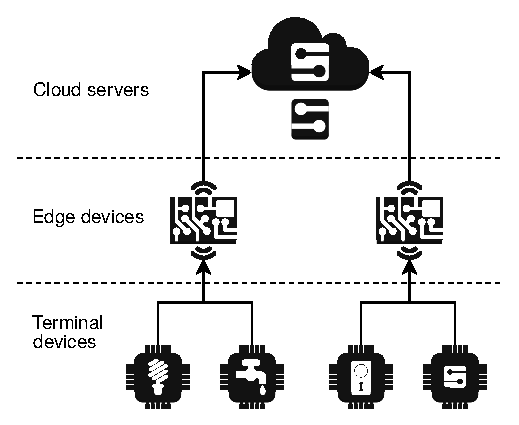
\includegraphics{figures/iot-hierarchy.drawio.eps}
\caption{Архитектура сложной системы.} \label{fig1}
\end{figure}

Такая архитектура дает гибкость сбора данных.
В случае проблем с соединением между конечным устройством и облаком, данные могут быть буферизованы на граничном устройстве и переотправлены позднее, когда подключение восстановится. Следовательно, такое граничное устройство должно обладать возможностью сбора и хранения данных от конечных устройств на случай таких проблем. Однако, такие граничные устройства не обладают достаточной аппаратной мощностью для использования полноценной СУБД, поэтому возможность буферизации данных должна быть встроена в одно из тех приложений, которые уже запущены на этом граничном устройстве. Следовательно, появляется необходимость во встраивании системы хранения временных рядов в подобные приложения. Здесь следует сделать предположение о том, что подобное приложение написано на языке программирования Go, потому что этот язык является сбалансированным с точки зрения сложности разработки, будучи более простым, чем C/С++, и с точки зрения производительности, будучи менее требовательным к ресурсам, чем Python. Также этот язык программирования был выбран потому, что он является стандартом в той предметной области, в которой работает автор этой статьи.

\subsection{Встраиваемые системы хранения}

Традиционно, для хранения данных в приложении используется либо какая-нибудь структура данных, располагающаяся целиком в оперативной памяти, либо встраиваемая СУБД. Однако в случае, когда важно не терять данные в случае отключения питания, структуры данных, хранящиеся в оперативной памяти, не подходят, а встраиваемые СУБД гораздо медленнее с точки зрения доступа к данным. В статье описывается подход хранения данных, использующий структуру под названием LSM-дерево. Такой подход похволяет добиться хранения данных на диске, не сильно теряя в производительности по сравнению с in-memory структурами данных.